%\documentclass[12pt, a4paper]{article}
\documentclass[runningheads]{llncs}
\usepackage{graphicx}
\usepackage{wrapfig}
\usepackage{subfigure}
\usepackage{multirow}
\usepackage{hyperref}
\usepackage{amsmath}
\usepackage{amssymb}
\usepackage{capt-of}
% \usepackage{ngerman}
\usepackage[ansinew]{inputenc}
\usepackage[left=2.5cm,top=2.5cm]{geometry}

\renewcommand\UrlFont{\color{blue}\rmfamily}

\begin{document}

\title{The effect of commen network problems on students academic performance in an elearning-Environment \thanks{Supported by Goethe University Frankfurt a. Main}}

\author{Lucas Laub\inst{1}\orcidID{6621331} \and
Alexander Perekhrest \inst{2}\orcidID{6379748}}

\institute{Goethe University Frankfurt, 60323 Frankfurt a. Main, Germany.}

\maketitle

\begin{abstract}
In the current light of the pandemic the worldwide use
of eLearning-Software experienced an unpresented boom.
We state the question how commen network problems influence
the academic performance in an eLearning-Environment.
To provide answers an online questionnaire with deliberate
technical difficulties was constructed. Evaluating the performance
of the test and controll group did not show any significant
differences.
\keywords{eLearning  \and Online-Learning \and academic performance.}
\end{abstract}


\section{Introduction}
When trying to transfer an already existing method on a relatively new platform, 
it's important to know the things that come with being on such a platform and the 
possible influences those things might have on the method.\\\\

In day-to-day usage of online platforms and services it's not uncommon to face some 
issues, whether it's execution, connectivity and so on. E-Learning-platforms are not 
particularly different to those. Therefore, we want to discuss, in this paper, to 
which extent these problems can influence the test-results of being on such an 
'issue-infected' platform in contrast to a well running platform with no issues.\\\\

We tried to focus on the most frequent issues we faced in our experience of browsing 
on different platforms, which are defined by HTTP-status-codes, like 400 (Bad Request), 401 
(Unauthorized), 403 (Forbidden), 404 (Not Found), 408 (Request Timeout), as mostly being 'client-errors'.\\\\

\section{Materials and Methodes}
\subsection{Preperations}
The experiment was conducted by creating a software implementing Fig.~\ref{fig1}.
This software allowed the tracking of {\itshape technical problems} introduced by
the software itself as well as the points and answers scored by each participant.
Additianaly a room with an adequat number of computers with a fiber-connection
to the server are needed, to rule out uncontrolled network problems.
Half of the cumputers are manipulated and simulate the network problems with the
use of the software.

\begin{figure}
    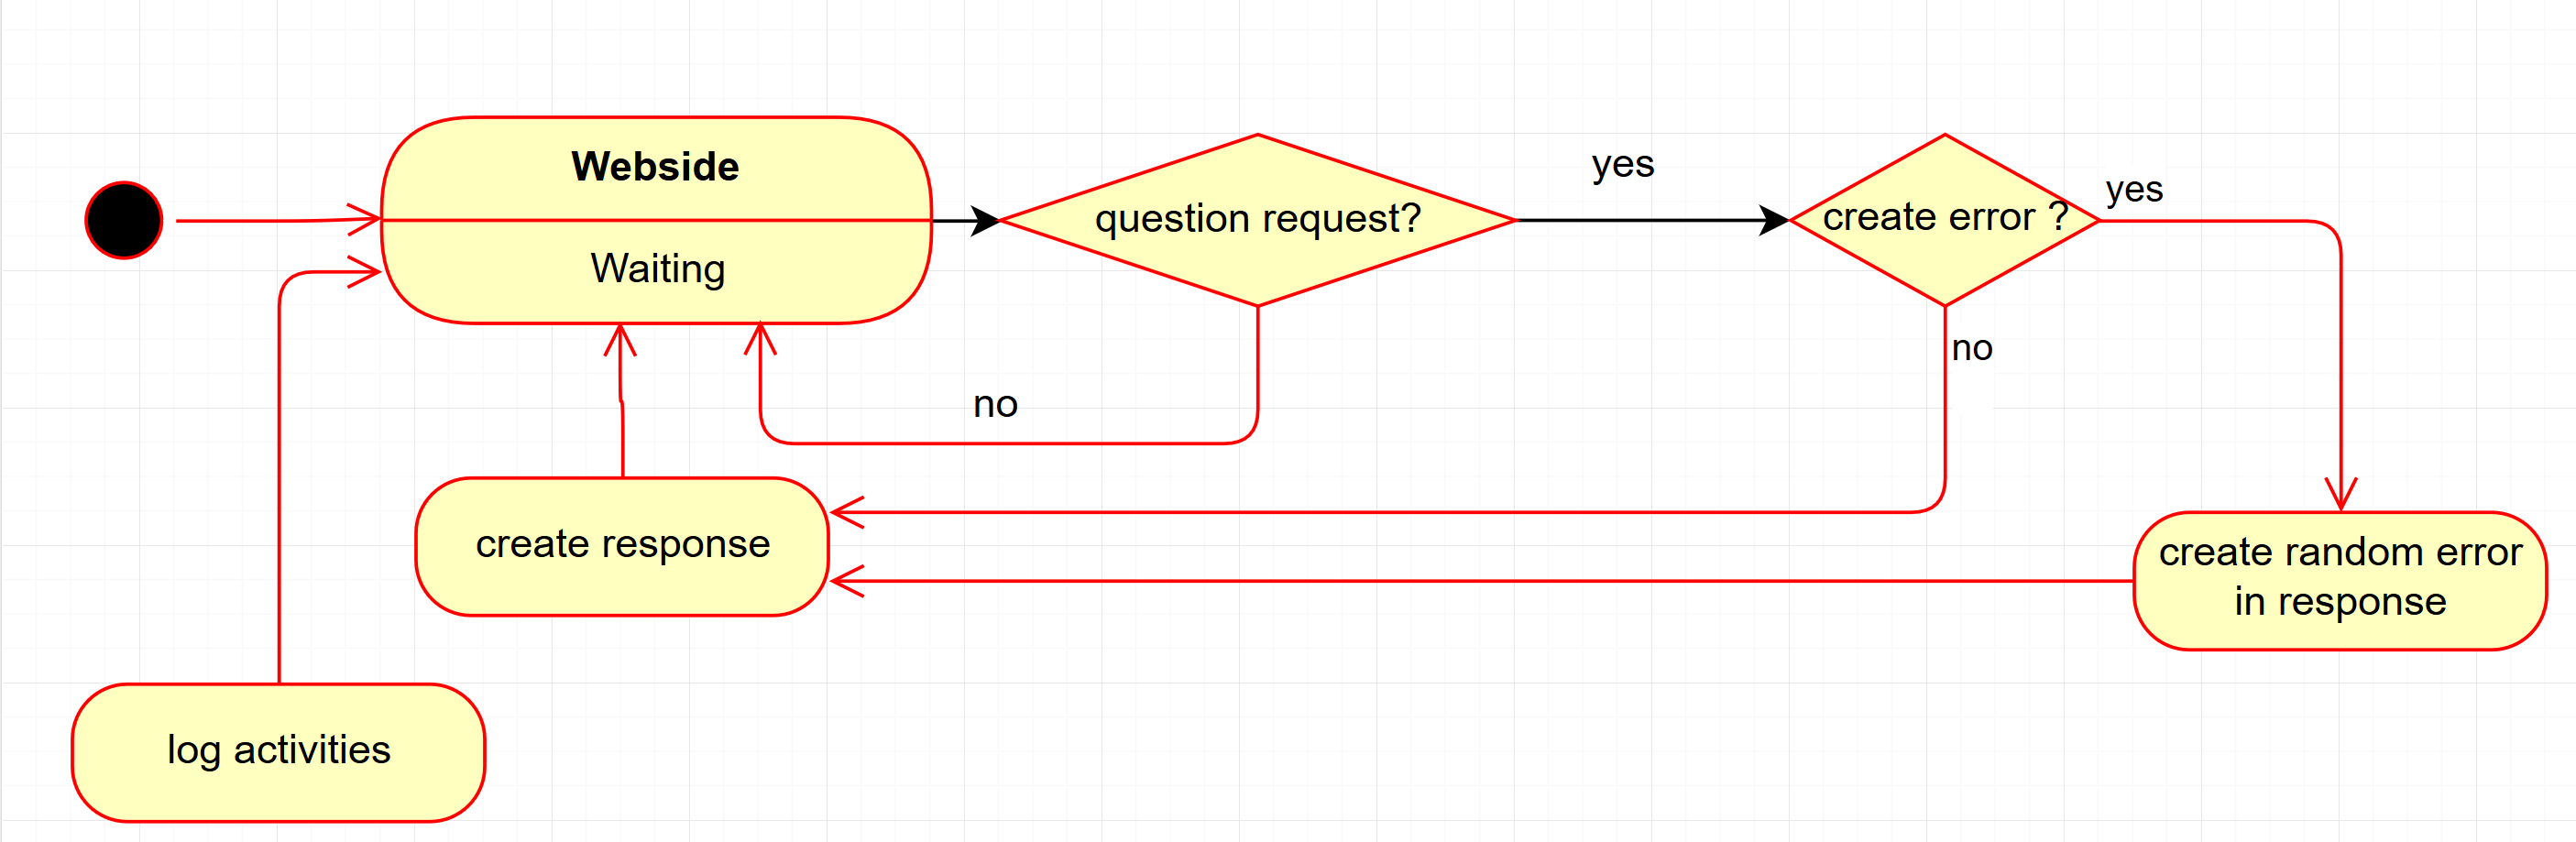
\includegraphics[width=\textwidth]{UML Prototyp.PNG}
    \caption{A logic flow chart , representing how an implementation could operate.
    The black circle is the user interacting with the software. The webside would
    consist of two parts. A frontend handling user interaction and the creation of {\itshape bugs}.
    The backend responsible for saving the collected data and ensuring the frontend
    remains operationale.} \label{fig1}
\end{figure}

\subsection{Participants}
The participants are students of the 5 grade and consist of two groups the controll group [CG] and
the test group [TG]. Each group is made up by 50 girls and 50 boys for a total of 200 participants.
It should be ensured that both groups prior to the experiment perform academicly similar, if not a
comparison post experiment will be difficult.

\newpage
\section{Results}
The results are displayed in chronological order of the analysis, there is
no emphisis on the significans given by the order itself.

\subsection{Controll Group vs Error Group}
\begin{figure}
    \begin{minipage}{0.45\textwidth}        
        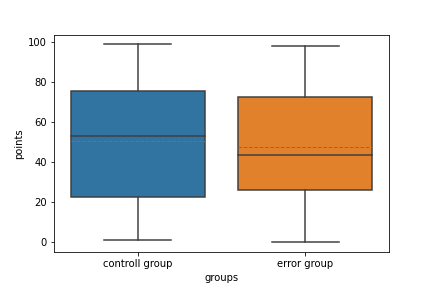
\includegraphics[width=\textwidth]{code/generate/all.png}
        \caption{The colored squares in the boxplot displays
        the upper and lower quartile of points earned by the controll group (50f/50m) and
        the error group (50f/50m).The green line marks the mean of all datapoints in the group.
        The gray line marks the median  of the given group.} \label{fig2}
    \end{minipage}
\hfill
\begin{minipage}{0.45\textwidth}
\captionof{table}{The calculated median, standart deviation and t, p-values
    for the controll group (50f/50m) the error group (50f/50m).
    The t,p-values were calculated by using a two-sided t-test.}
\begin{tabular}[]{| c | c | c |}
        \hline
        & controll group & error group \\
        \hline
        median & 53.0&43.5 \\
        \hline
        standart deviation & 29.278&29.826 \\
        \hline
        t-value & \multicolumn{2}{c|}{0.728} \\
        \hline
        p-value & \multicolumn{2}{c|}{0.467} \\
        \hline            
\end{tabular}
\end{minipage}
\end{figure}

\subsection{Controll Group Female vs Error Group Female}
\begin{figure}
    \begin{minipage}{0.45\textwidth}        
        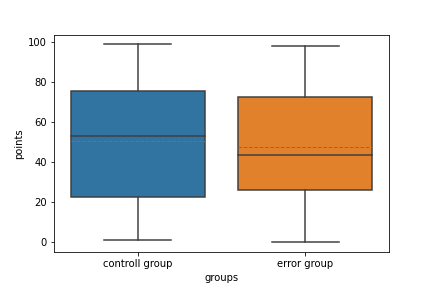
\includegraphics[width=\textwidth]{code/generate/all.png}
        \caption{The colored squares in the boxplot displays
        the upper and lower quartile of points earned by the controll group (50f) and
        the error group (50f).The green line marks the mean of all datapoints in the group.
        The gray line marks the median  of the given group.} \label{fig3}
    \end{minipage}
\hfill
\begin{minipage}{0.45\textwidth}
\captionof{table}{The calculated median, standart deviation and t, p-values
    for the controll group (50f) the error group (50f).
    The t,p-values were calculated by using a two-sided t-test.}
\begin{tabular}[]{| c | c | c |}
        \hline
        & controll group & error group \\
        \hline
        median & 55.5&40.0 \\
        \hline
        standart deviation & 27.85&30.933 \\
        \hline
        t-value & \multicolumn{2}{c|}{0.949} \\
        \hline
        p-value & \multicolumn{2}{c|}{0.345} \\
        \hline            
\end{tabular}
\end{minipage}
\end{figure}

\subsection{Controll Group Male vs Error Group Male }
\begin{figure}
    \begin{minipage}{0.45\textwidth}        
        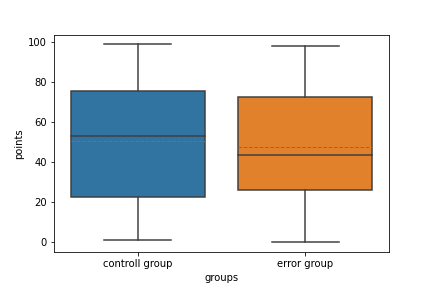
\includegraphics[width=\textwidth]{code/generate/all.png}
        \caption{The colored squares in the boxplot displays
        the upper and lower quartile of points earned by the controll group (50m) and
        the error group (50m).The green line marks the mean of all datapoints in the group.
        The gray line marks the median  of the given group.} \label{fig4}
    \end{minipage}
\hfill
\begin{minipage}{0.45\textwidth}
\captionof{table}{The calculated median, standart deviation and t, p-values
    for the controll group (50m) the error group (50m).
    The t,p-values were calculated by using a two-sided t-test.}
\begin{tabular}[]{| c | c | c |}
        \hline
        & controll group & error group \\
        \hline
        median & 52.5&50.5 \\
        \hline
        standart deviation & 30.638&28.495 \\
        \hline
        t-value & \multicolumn{2}{c|}{0.08} \\
        \hline
        p-value & \multicolumn{2}{c|}{0.936} \\
        \hline            
\end{tabular}
\end{minipage}
\end{figure}

\subsection{Controll Group vs Error Group}
\begin{figure}
    \begin{minipage}{0.45\textwidth}        
        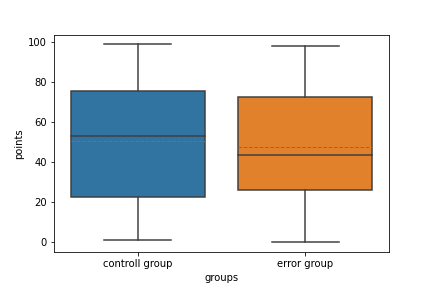
\includegraphics[width=\textwidth]{code/generate/all.png}
        \caption{The colored squares in the boxplot displays
        the upper and lower quartile of points earned by the controll group (50f) and
        the controll group (50m).The green line marks the mean of all datapoints in the group.
        The gray line marks the median  of the given group.} \label{fig5}
    \end{minipage}
\hfill
\begin{minipage}{0.45\textwidth}
\captionof{table}{The calculated median, standart deviation and t, p-values
    for the controll group (50f) the controll group (50m).
    The t,p-values were calculated by using a two-sided t-test.}
\begin{tabular}[]{| c | c | c |}
        \hline
        & controll group(f) & controll group(m) \\
        \hline
        median & 55.5&52.5 \\
        \hline
        standart deviation & 27.85&30.638 \\
        \hline
        t-value & \multicolumn{2}{c|}{0.101} \\
        \hline
        p-value & \multicolumn{2}{c|}{0.919} \\
        \hline            
\end{tabular}
\end{minipage}
\end{figure}

\subsection{Controll Group vs Error Group}
\begin{figure}
    \begin{minipage}{0.45\textwidth}        
        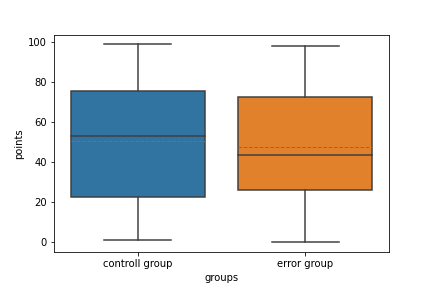
\includegraphics[width=\textwidth]{code/generate/all.png}
        \caption{The colored squares in the boxplot displays
        the upper and lower quartile of points earned by the error group (50f) and
        the error group (50m).The green line marks the mean of all datapoints in the group.
        The gray line marks the median  of the given group.} \label{fig6}
    \end{minipage}
\hfill
\begin{minipage}{0.45\textwidth}
\captionof{table}{The calculated median, standart deviation and t, p-values
    for the error group (50f) the error group (50m).
    The t,p-values were calculated by using a two-sided t-test.}
\begin{tabular}[]{| c | c | c |}
        \hline
        & error group & error group \\
        \hline
        median & 40.0&50.5 \\
        \hline
        standart deviation & 30.933&28.495 \\
        \hline
        t-value & \multicolumn{2}{c|}{- 0.759} \\
        \hline
        p-value & \multicolumn{2}{c|}{0.45} \\
        \hline            
\end{tabular}
\end{minipage}
\end{figure}

\subsection{Controll Group vs Error Group}
\begin{figure}
    \begin{minipage}{0.45\textwidth}        
        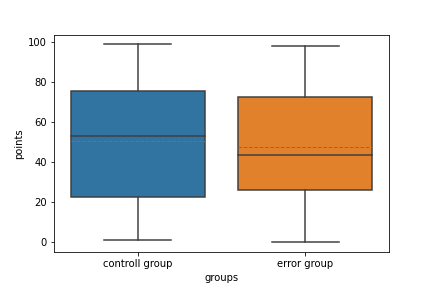
\includegraphics[width=\textwidth]{code/generate/all.png}
        \caption{The colored squares in the boxplot displays
        the upper and lower quartile of points earned by the controll group (50f) and
        the error group (50m).The green line marks the mean of all datapoints in the group.
        The gray line marks the median  of the given group.} \label{fig7}
    \end{minipage}
\hfill
\begin{minipage}{0.45\textwidth}
\captionof{table}{The calculated median, standart deviation and t, p-values
    for the controll group (50f) the error group (50m).
    The t,p-values were calculated by using a two-sided t-test.}
\begin{tabular}[]{| c | c | c |}
        \hline
        & controll group & error group \\
        \hline
        median & 55.5&50.5 \\
        \hline
        standart deviation & 27.85&28.495 \\
        \hline
        t-value & \multicolumn{2}{c|}{0.19} \\
        \hline
        p-value & \multicolumn{2}{c|}{0.85} \\
        \hline            
\end{tabular}
\end{minipage}
\end{figure}

\subsection{Controll Group vs Error Group}
\begin{figure}
    \begin{minipage}{0.45\textwidth}        
        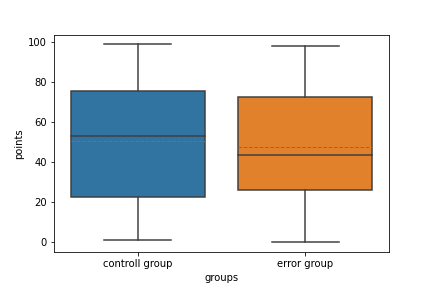
\includegraphics[width=\textwidth]{code/generate/all.png}
        \caption{The colored squares in the boxplot displays
        the upper and lower quartile of points earned by the controll group (50m) and
        the error group (50f).The green line marks the mean of all datapoints in the group.
        The gray line marks the median  of the given group.} \label{fig8}
    \end{minipage}
\hfill
\begin{minipage}{0.45\textwidth}
\captionof{table}{The calculated median, standart deviation and t, p-values
    for the controll group (50m) the error group (50f).
    The t,p-values were calculated by using a two-sided t-test.}
\begin{tabular}[]{| c | c | c |}
        \hline
        & controll group & error group \\
        \hline
        median & 52.5&40.0 \\
        \hline
        standart deviation & 30.638&30.933 \\
        \hline
        t-value & \multicolumn{2}{c|}{0.81} \\
        \hline
        p-value & \multicolumn{2}{c|}{0.42} \\
        \hline            
\end{tabular}
\end{minipage}
\end{figure}






\section{Discussion}
\section{Conclusion}
\section{Refernces}
\end{document}
